\documentclass[aspectratio=169,10pt]{beamer}

\usetheme{metropolis}
\usepackage{appendixnumberbeamer}
\usepackage{booktabs}
\usepackage{colortbl}
\usepackage{tikz}
\usepackage{pgfplots}
\usepackage{xcolor}
\usepackage{fontspec}
\usepackage[font=footnotesize]{caption}
\usetikzlibrary{positioning,arrows.meta,shapes.geometric,fit,backgrounds,calc}
\pgfplotsset{compat=1.18}

% ---- Harvard crimson palette
\definecolor{crimson}{HTML}{A51C30}
\definecolor{crimsonDark}{HTML}{7A1424}
\definecolor{ink}{HTML}{1E293B}
\definecolor{soft}{HTML}{F1F5F9}
\definecolor{rule}{HTML}{E2E8F0}
\definecolor{ok}{HTML}{16A34A}
\definecolor{warn}{HTML}{D97706}
\definecolor{bad}{HTML}{DC2626}

\setbeamercolor{normal text}{fg=ink}
\setbeamercolor{alerted text}{fg=crimson}
\setbeamercolor{frametitle}{bg=crimson, fg=white}
\setbeamercolor{progress bar}{fg=crimson, bg=rule}
\setbeamercolor{title separator}{fg=crimson}
\setbeamercolor{progress bar in section page}{fg=crimson, bg=rule}

\title{Cache-Informed Prompting for\\Recursive Language Models}
\subtitle{}
\author{Fucheng Warren Zhu}
\institute{CS2640 · Spring 2026}
\date{}

\begin{document}

% =====================================================================
\begin{frame}[plain]
  \titlepage
\end{frame}

% =====================================================================
\begin{frame}{Context is a cache}
\begin{columns}[T,onlytextwidth]
\column{0.55\textwidth}
\begin{itemize}\setlength{\itemsep}{0.7em}
  \item LLMs come with a 200K-token cache called \emph{context}.
  \item When it fills, we need a policy for eviction.
  \item Popular policies are not very principled:
    \begin{itemize}
      \item drop-oldest
      \item summarize-and-collapse
      \item persist to filesystem, keep an index in cache
    \end{itemize}
  \item This course covered better answers: LRU, LFU, S3-FIFO, SIEVE,
        admission control.
  \item \textbf{Question.} Can we just tell the model to use a real policy?
\end{itemize}
\column{0.45\textwidth}
\centering
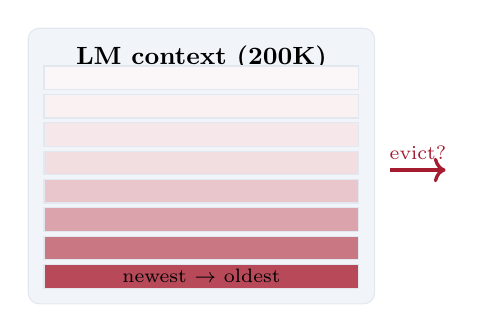
\begin{tikzpicture}[font=\footnotesize]
  \draw[rounded corners=4pt, fill=soft, draw=rule] (0,0) rectangle (4.4,3.5);
  \node[anchor=north, font=\small\bfseries] at (2.2,3.4) {LM context (200K)};
  \foreach \i/\c in {0/crimson!80, 1/crimson!60, 2/crimson!40, 3/crimson!25, 4/crimson!15, 5/crimson!10, 6/crimson!6, 7/crimson!4} {
    \draw[fill=\c, draw=rule] (0.2,0.2 + 0.36*\i) rectangle (4.2, 0.5 + 0.36*\i);
  }
  \node at (2.2, 0.36) {\scriptsize newest $\to$ oldest};
  \draw[->, very thick, crimson] (4.6, 1.7) -- (5.3, 1.7) node[midway, above] {\scriptsize evict?};
\end{tikzpicture}
\end{columns}
\end{frame}

% =====================================================================
\begin{frame}{Recursive Language Models}
\small Zhang, Kraska \& Khattab, arXiv:2512.24601 (2026)
\vspace{0.4em}
\centering
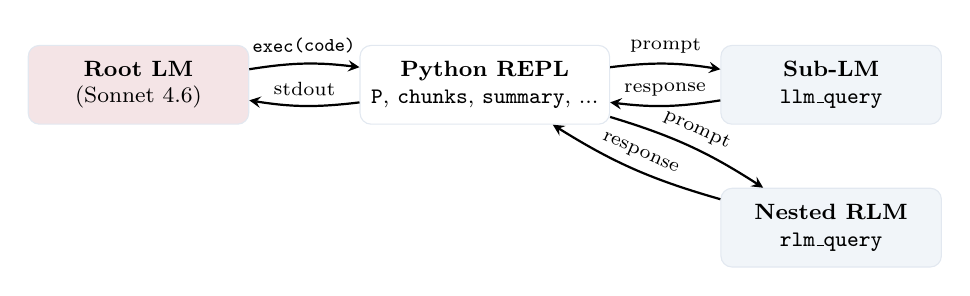
\begin{tikzpicture}[
    node distance=10mm,
    box/.style={rounded corners=4pt, draw=rule, fill=white, minimum height=10mm, font=\footnotesize, align=center, inner sep=4pt},
    label/.style={font=\scriptsize, midway, above, sloped},
    every edge/.append style={->, >=stealth, thick}
  ]
  \node[box, fill=crimson!12, minimum width=28mm] (root) {\textbf{Root LM}\\(Sonnet 4.6)};
  \node[box, right=14mm of root, minimum width=28mm] (repl) {\textbf{Python REPL}\\\texttt{P}, \texttt{chunks}, \texttt{summary}, ...};
  \node[box, right=14mm of repl, minimum width=28mm, fill=soft] (sub1) {\textbf{Sub-LM}\\\texttt{llm\_query}};
  \node[box, below=8mm of sub1, minimum width=28mm, fill=soft] (sub2) {\textbf{Nested RLM}\\\texttt{rlm\_query}};

  \draw (root) edge[bend left=8] node[label]{\texttt{exec(code)}} (repl);
  \draw (repl) edge[bend left=8] node[label]{stdout} (root);
  \draw (repl) edge[bend left=8] node[label]{prompt} (sub1);
  \draw (sub1) edge[bend left=8] node[label]{response} (repl);
  \draw (repl) edge[bend left=8] node[label]{prompt} (sub2);
  \draw (sub2) edge[bend left=8] node[label]{response} (repl);
\end{tikzpicture}
\vspace{0.4em}
\begin{itemize}\setlength{\itemsep}{0.2em}
  \item User prompt lives in the REPL as variable \texttt{P} --- not in the context window.
  \item Root LM sees only metadata (length, prefix) and writes code to inspect / slice it.
  \item Variables persist; \texttt{del} evicts. The LM runs until it emits \texttt{FINAL(answer)}.
\end{itemize}
\end{frame}

% =====================================================================
\begin{frame}{Paper results --- RLM lifts every benchmark}
\small Zhang+Kraska+Khattab 2026, Table 1 (GPT-5 row). Accuracy (\%).
\vspace{0.4em}
\centering
\renewcommand{\arraystretch}{1.25}
\footnotesize
\begin{tabular}{@{}l c c c c@{}}
\toprule
\textbf{Method} & \textbf{CodeQA} & \textbf{BrowseComp+\,(1K)} & \textbf{OOLONG} & \textbf{OOLONG-Pairs} \\
\textit{\scriptsize Task length} & \textit{\scriptsize 23K--4.2M} & \textit{\scriptsize 6M--11M} & \textit{\scriptsize 131K} & \textit{\scriptsize 32K} \\
\midrule
Base Model              & 24.0$^*$ & 0.0$^*$  & 44.0 & 0.1 \\
CodeAct + BM25          & 22.0$^*$ & 51.0     & 38.0 & 24.7 \\
Summary agent           & 58.0     & 70.5     & 46.0 & 0.1 \\
\rowcolor{crimson!10}\textbf{RLM} & \textbf{62.0} & \textbf{91.3} & \textbf{56.5} & \textbf{58.0} \\
RLM (no sub-calls)      & 58.0 & 88.0 & 36.0 & 43.9 \\
\bottomrule
\end{tabular}
\vspace{0.2em}\\
{\scriptsize $^*$ = method (sometimes) ran into input context limits.}

\vspace{0.6em}
\begin{itemize}\setlength{\itemsep}{0.2em}
  \item RLM scaffold lifts every benchmark over every other method.
  \item Biggest lift: OOLONG-Pairs (0.1\% $\to$ 58\%).
  \item \emph{Recursion} matters: disabling sub-calls drops OOLONG-Pairs 58 $\to$ 43.9.
  \item \textbf{Cost-comparable to base model.} RLM pays for what it
        \emph{reads}, not what's \emph{available} --- on long inputs you only
        need a small fraction. Risk: confused trajectories can recurse a long
        way before terminating, so cost has high variance.
  \item Even GPT-5 RLM never saturates --- room for further work on top.
\end{itemize}
\end{frame}

% =====================================================================

% =====================================================================
\begin{frame}{Experimental design}
\textbf{Five benchmarks (same set as the paper):}
\begin{itemize}\setlength{\itemsep}{0.05em}
  \item \textbf{S-NIAH} --- 2K--262K filler with one injected key. Retrieval.
  \item \textbf{LongBench-v2 CodeQA} --- 23K--4.2M tokens of code, 4-way MC.
  \item \textbf{BrowseComp+ (1K)} --- 6M--11M tokens, multi-hop over 1K docs.
  \item \textbf{OOLONG} (trec\_coarse) --- 131K tokens, semantic aggregation.
  \item \textbf{OOLONG-Pairs} --- 32K tokens, quadratic pairwise reasoning.
\end{itemize}

\vspace{0.5em}
\textbf{Eight methods:}
\begin{itemize}\setlength{\itemsep}{0.05em}
  \item \textbf{Baselines (4):} \texttt{direct}, \texttt{summary\_agent},
        \texttt{codeact\_bm25}, and \alert{\texttt{rlm\_a0}} (vanilla RLM, the RLM baseline).
  \item \textbf{Treatment arms (4):} a single cache-hint block appended to
        the RLM system prompt --- see next slide.
\end{itemize}

\vspace{0.4em}
Sonnet 4.6, via the Agent SDK over a Max-subscription OAuth token.
\end{frame}

% =====================================================================
\begin{frame}{The four treatment arms}
\small Each arm appends a single hint block to the upstream RLM system prompt.
\vspace{0.4em}
\renewcommand{\arraystretch}{1.4}
\footnotesize
\begin{tabular}{@{}p{1.0cm} p{2.6cm} p{8.5cm}@{}}
\toprule
\textbf{Arm} & \textbf{Policy} & \textbf{What it tells the model} \\
\midrule
\textbf{A1} & LRU & "When you must evict, prefer to \texttt{del} the variable you
                   have not touched recently." Tests temporal locality. \\
\textbf{A2} & S3-FIFO  & "New variables are on probation. Promote to a main
                   set only on re-reference; evict the rest. Track recently
                   evicted in a ghost set." Tests one-hit-wonder filtering. \\
\textbf{A3} & SIEVE    & "Walk variables in creation order. On each pass,
                   evict the first one not re-referenced since last pass."
                   Tests lazy promotion. \\
\textbf{A4} & theory primer & A short primer on \emph{retention vs.\
                   reconstruction cost}, the LRU/LFU/S3-FIFO/SIEVE menu, and
                   admission filtering. This is a non-prescriptive
                   decision framework. \\
\bottomrule
\end{tabular}

\vspace{0.6em}
\textbf{The control} is \texttt{rlm\_a0} (vanilla RLM with empty suffix).
\textbf{What we want to learn:} does any of A1--A3 (directive) outperform
\texttt{rlm\_a0}? Does A4 (framework) behave differently from the directive
arms?
\end{frame}

% =====================================================================
\begin{frame}{Preliminary results --- S-NIAH and CodeQA}
\small We first ran on shorter context tasks as a preliminary investigation.

\vspace{0.4em}
\begin{center}
\renewcommand{\arraystretch}{1.1}
\scriptsize
\begin{tabular}{@{}l c c@{}}
\toprule
\textbf{Method} & \textbf{S-NIAH} (retrieval, 2K--262K) & \textbf{CodeQA} (reasoning, $\sim$100K) \\
\midrule
direct                & 1.00 & 1.00 \\
summary\_agent        & 1.00 & 0.33 \\
codeact + BM25        & 0.43 & 0.33 \\
\midrule
\rowcolor{crimson!5}rlm\_a0 (vanilla RLM) & 1.00 & 0.50 \\
A1 (LRU)              & 0.67 & 0.00 \\
A2 (S3-FIFO)          & \alert{0.20} & 0.67 \\
A3 (SIEVE)            & \alert{0.20} & --- \\
A4 (theory primer)    & 0.60 & 1.00 \\
\bottomrule
\end{tabular}
\end{center}

\vspace{0.4em}
\footnotesize\textbf{Observations:}
\begin{itemize}\setlength{\itemsep}{0.05em}
  \item Directive arms (A2, A3) collapse on retrieval --- 1.00 $\to$ 0.20.
  \item Even the gentler primer (A4) drops to 0.60 at higher tiers.
  \item On reasoning the directive arms \emph{help}: A2 lifts CodeQA 0.50 $\to$ 0.67.
  \item Vanilla RLM is the strongest cache-aware method on retrieval; no treatment arm beats it.
\end{itemize}
\end{frame}

% =====================================================================
\begin{frame}{Findings and next steps}
\textbf{Preliminary results --- we need much more experimentation on top to validate.}
\vspace{0.6em}
\begin{enumerate}[(a)]\setlength{\itemsep}{0.5em}
  \item \alert{Prompt hints can manufacture failures.}
        On S-NIAH directive arms led the model to evict its own answer.
        1.00 $\to$ 0.20.
  \item \alert{Same hints, opposite signs across tasks.}
        The arm that hurt S-NIAH lifts CodeQA 0.50 $\to$ 0.67. Hints act
        as a prior --- helps when it matches the task, hurts when it doesn't.
  \item \alert{The decision space is enormous.} A few hundred prompt tokens
        may not encode the right behavior across all task structures. The
        right layer might be the runtime, not the prompt.
  \item \alert{Efficiency is missing.} We tracked accuracy only. Open question:
        \textbf{how can eviction policies be KV-cache aware?} Policies that
        preserve the prefix keep KV reuse cheap.
\end{enumerate}

\end{frame}

\end{document}
